\documentclass[../../main.tex]{subfiles}
\begin{document}
Sei wieder $K$ ein Körper.

\section[tocentry={Quotientenvektorräume}]{Quotientenvektorräume {\small [$\to$ §\ref{1.3}, §\ref{2.3}, §\ref{3.3}]}}

\begin{df}\label{8.1.1}
[$\to$ \ref{2.3.1}, \ref{3.3.1}] Sei $V$ ein $K$-Vektorraum. Eine \emph{Kongruenzrelation}\index{Relation@{\bf Relation}!Kongruenzrelation ($\equiv$)} auf $V$ ist eine Kongruenzrelation $\equiv$ auf der additiven Gruppe von $V$, für die gilt:
\[\forall v,w\in V:\forall\lambda\in K:(v\equiv w \Longrightarrow \lambda v \equiv \lambda w).\]
\end{df}

\begin{bem}\label{8.1.2}
[$\to$ \ref{2.3.2}, \ref{3.3.2}] Definition \ref{8.1.1} wurde gerade so gemacht, dass
\begin{align*}
K \times V/{\equiv} & \to V/{\equiv}\\
(\lambda, \overline{v}) & \mapsto \overline{\lambda v} & (\lambda\in K, v\in V)
\end{align*}
wohldefiniert ist.
\end{bem}

\begin{satdef}\label{8.1.3}
{\rm[$\to$ \ref{2.3.3}, \ref{3.3.3}]} Ist $V$ ein $K$-Vektorraum und $\equiv$ eine Kongruenzrelation auf $V$, so wird die Quotientengruppe $V/{\equiv}$ vermöge der Skalarmultiplikation definiert durch
$$\lambda \overline{v} := \overline{\lambda v}\quad (\lambda \in K, v\in V)$$
zu einem $K$-Vektorraum ("`Quotientenvektorraum"')\index{Relation@{\bf Relation}!Kongruenzrelation ($\equiv$)!Quotientenvektorraum}.
\end{satdef}
\begin{proof}
direktes Nachrechnen, von (V), \vecN, \vecD, (D') aus \ref{6.1.1}.
\end{proof}

\begin{sat}\label{8.1.4}
{\rm[$\to$ \ref{2.3.6}, \ref{3.3.6}]} Sei $V$ ein Vektorraum. Die Zuordnungen
\begin{align*}
\equiv & \mapsto \overline{0}\\
\equiv_U & \mapsfrom U
\end{align*}
vermitteln eine Bijektion zwischen der Menge der Kongruenzrelationen auf $V$ und der Menge der Unterräume auf $V$.
\end{sat}
\begin{proof}
Übung (vgl. \ref{3.3.6}).
\end{proof}

\begin{nt}\label{8.1.5}
[$\to$ \ref{2.3.7}, \ref{3.3.7}] Sei $V$ ein Vektorraum und $U$ ein Unterraum von $V$.
\[V/U:= V/{\equiv_U}\qquad\text{"`$V$ modulo $U$"'}\]
\end{nt}

\begin{bsp}\label{8.1.6}
\begin{enumerate}[\normalfont(a)]
\item $\R^2/\spann{\cvec{2\\1}}$ besteht aus allen Geraden in der Ebene mit Steigung $\frac{1}{2}$.

\begin{center}
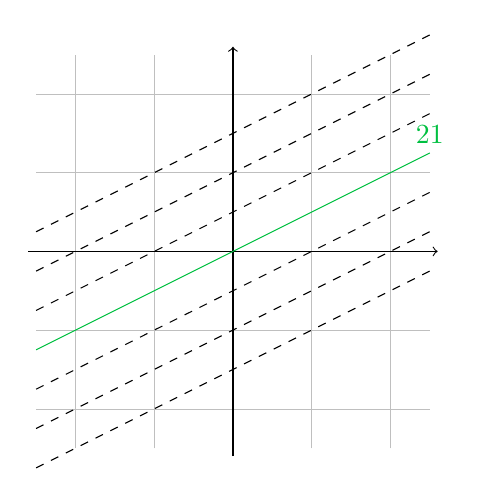
\begin{tikzpicture}[domain=-2.5:2.5]
\draw[very thin, gray!50] (-2.5,-2.5) grid (2.5,2.5);
\draw[->] (-2.6,0) -- (2.6,0) node[right]{$\R$};
\draw[->] (0,-2.6) -- (0,2.6) node[above]{$\R$};

\foreach \y in {-1.5,-1,-.5,.5,1,1.5}
	\draw[dashed] plot (\x,.5 * \x + \y);

\draw[green!75!blue] plot (\x,.5 * \x) node[above]{$\spann{\cvec{2\\1}}$};
\end{tikzpicture}
\end{center}
\item $\F_5^2/\spann{\cvec{2\\1}} = \left\{\underbrace{\overline{0}}_{\tikz[scale = .5, baseline] \draw (0,0) circle (.2);},\underbrace{\overline{\cvec{1\\0}}}_{\tikz[scale = .5, baseline] \draw (-.14, -.14) -- (.14, -.14) -- (0, .2) -- cycle;},\underbrace{\overline{\cvec{2\\0}}}_{\tikz[scale = .5, baseline] \draw (-.2, -.2) rectangle (.2, .2);},\underbrace{\overline{\cvec{3\\0}}}_{\tikz[scale = .5, baseline] \filldraw (-.14, -.14) -- (.14, -.14) -- (0, .2) -- cycle;},\underbrace{\overline{\cvec{4\\0}}}_{\tikz[scale = .5, baseline] \filldraw (-.2, -.2) rectangle (.2, .2);}\right\}$
\begin{center}
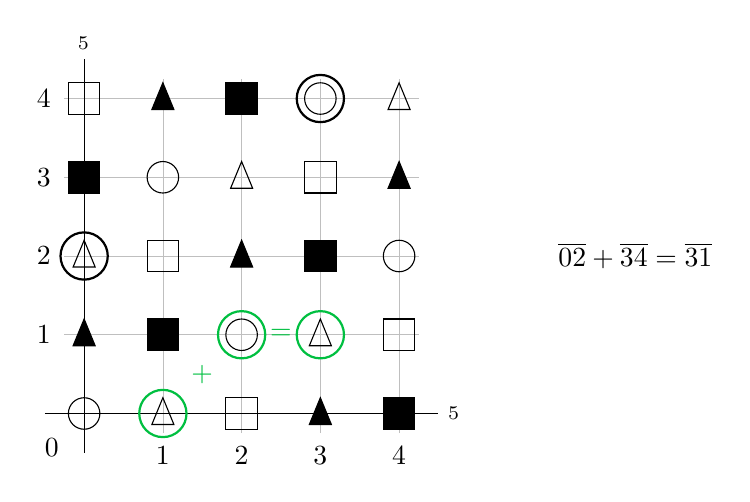
\begin{tikzpicture}
\draw[very thin, gray!50] (-.25,-.25) grid (4.25,4.25);
\draw (-.5,0) -- (4.5,0) node[right]{$\F_5$};
\draw (0,-.5) -- (0,4.5) node[above]{$\F_5$};

\foreach \x in {1,...,4}{
	\draw (\x,-.3) node[anchor = north]{$\x$};
	\draw (-.3,\x) node[anchor = east]{$\x$};
}
\draw (-.2,-.2) node[anchor = north east]{$0$};

\foreach \x in {0,...,4}{
	\pgfmathMod{\x * 2}{5};
	\draw (\pgfmathresult, \x) circle (.2);
}

\foreach \x in {0,...,4}{
	\pgfmathsetmacro\y{Mod(\x * 2 + 1, 5)};
	\draw (\y - .14, \x - .14) -- (\y + .14, \x - .14) -- (\y, \x + .2) -- cycle;
}

\foreach \x in {0,...,4}{
	\pgfmathsetmacro\y{Mod(\x * 2 + 2, 5)};
	\draw (\y - .2, \x - .2) rectangle (.2+ \y, .2+\x);
}

\foreach \x in {0,...,4}{
	\pgfmathsetmacro\y{Mod(\x * 2 + 3, 5)};
	\filldraw (\y - .14, \x - .14) -- (\y + .14, \x - .14) -- (\y, \x + .2) -- cycle;
}

\foreach \x in {0,...,4}{
	\pgfmathsetmacro\y{Mod(\x * 2 + 4, 5)};
	\filldraw (\y - .2, \x - .2) rectangle (.2+ \y, .2+\x);
}

\draw[thick] (0,2) circle (.3);
\draw[thick] (3,4) circle (.3);
\draw[green!75!blue, thick] (1,0) circle (.3);
\draw[green!75!blue, thick] (2,1) circle (.3);
\draw[green!75!blue, thick] (3,1) circle (.3);
\draw[green!75!blue] (1.5,.5) node{$+$};
\draw[green!75!blue] (2.5,1) node{$=$};
\draw (7,2) node{$\overline{\cvec{0\\2}}+\overline{\cvec{3\\4}} = \overline{\cvec{3\\1}}$};
\end{tikzpicture}
\end{center}
\end{enumerate}
\end{bsp}

\begin{pro}\label{8.1.7}
{\rm[$\to$ \ref{2.3.10}, \ref{2.3.13}, \ref{3.3.15}, \ref{imfsubring}]} Seien $V$ und $W$ $K$-Vektorräume und $f\colon V\to W$ linear. Dann ist $\equiv_f$ eine Kongruenzrelation auf $V$ und $\ker f$ ein Unterraum von $V$. Weiter ist $\im f$ ein Unterraum von $W$.
\end{pro}
\begin{proof}
Übung.
\end{proof}

\begin{pro}\label{8.1.8}
Sei $V$ ein $K$-Vektorraum und $U$ ein Unterraum von $V$. Dann ist die kanonische Surjektion\index{Vektorraum@{\bf Vektorraum}!Unterraum!kanonische Surjektion} $V\to V/U$ linear.
\end{pro}
\begin{proof}
Übung.
\end{proof}

\red{Bis hierher sollten wir am 13. Januar kommen.}

\begin{sat}[Homomorphiesatz für Vektorräume]\label{8.1.9}
{\rm[$\to$ \ref{2.3.11}, \ref{3.3.16}]} Seien $V$ und $W$ $K$-Vektorräume, $U$ ein Unterraum von $V$ und $f\colon V\to W$ linear mit $U\subseteq \ker f$.
\begin{enumerate}[\rm(a)]
\item Es gibt genau eine Abbildung $\overline{f}: V/U\to W$ mit $\overline{f}(\overline{v})= f(v)$ für alle $v\in V$. Diese Abbildung ist linear.
\item $\overline{f} \text{ injektiv }\iff U = \ker f$
\item $\overline{f} \text{ surjektiv } \iff f \text{ surjektiv}$.
\end{enumerate}
\end{sat}
\begin{proof}
folgt fast alles aus \ref{2.3.11}. Nur noch zu zeigen [$\to$ \ref{6.3.1}]:
\[\forall v\in V:\forall \lambda\in K:\overline{f}(\lambda \overline{v}) = \lambda\overline{f}(\overline{v}).\] Sei also $v\in V$ und $\lambda\in K$. Dann $\overline{f}(\lambda\overline{v}) = \overline{f}(\overline{\lambda v}) = f(\lambda v) = \lambda f(v) = \lambda\overline{f}(\overline{v})$.
\end{proof}

\begin{kor}[Isomorphiesatz für Vektorräume]\label{8.1.10}
{\rm[$\to$ \ref{2.3.14}, \ref{isothmring}]} Seien $V$ und $W$ $K$-Vektorräume und $f\colon V\to W$ linear. Dann ist $\overline{f}:V/\ker f\to \im f$ definiert durch $\overline{f}(\overline{v})= f(v)$ für $v\in V$ ein $K$-Vektorraumisomorphismus. Insbesondere $V/\ker f\cong \im f$.
\end{kor}

\begin{lem}\label{8.1.11}
Sei $V$ ein Vektorraum und $U$ ein Unterraum von $V$ mit Basis \\
$(u_1,\ldots,u_m)$. Seien $v_1,\ldots,v_n\in V$. Dann $$(\overline{v_1},\ldots,\overline{v_n})\text{ Basis von }V/U\iff (u_1,\ldots,u_m,v_1,\ldots,v_n)\text{ Basis von }V.$$ Insbesondere $\dim(U)+\dim(V/U) = \dim(V)$ falls $\dim V< \infty$.
\end{lem}
\begin{proof}
$K:=$ Grundkörper von $V$ [$\to$ \ref{6.1.2}(c)].
\begin{itemize}
\item["`$\Longrightarrow$"'] Sei $(\overline{v_1},\ldots,\overline{v_n})$ Basis von $V/U$. Zu zeigen:
\begin{enumerate}[\normalfont(a)]
\item $u_1,\ldots,u_m,v_1,\ldots,v_n$ linear unabhängig in $V$
\item $V = \spann{u_1,\ldots,u_m,v_1,\ldots,v_n}$
\end{enumerate}
\begin{enumerate}[Zu (a).]
\item Seien $\lambda_i,\mu_i\in K$ mit $\sum_{i = 1}^{m}\lambda_iu_i+\sum_{j = 1}^{n}\mu_jv_j = 0$. Zu zeigen: $\lambda_i = \mu_i = 0$.

Aus $\sum_{j = 1}^{m}\mu_j\overline{v_j} = \overline{\sum_{i = 1}^{m}\lambda_i u_i+\sum_{j = 1}^{n}\mu_jv_j} = 0$ folgt $\mu_j = 0$ für alle $j$, da $\overline{v_1},\ldots,\overline{v_n}$ linear unabhängig.

Da $u_1,\ldots,u_m$ auch linear unabhängig, folgt $\lambda_i = 0$ für alle $i$.
\item Sei $v\in V$. Zu zeigen: $\exists\lambda_i, \mu_i\in K: v = \sum_{i = 1}^{m}\lambda_iu_i+\sum_{j = 1}^{n}\mu_jv_j$. Da $\overline{v_1},\ldots,\overline{v_n}$ den Vektorraum $V/U$ aufspannen, gibt es $\mu_j\in K$ mit $\overline{v} = \sum_{j = 1}^{n}\mu_i,\overline{v_j}$. Es folgt $v-\sum_{j = 1}^{n}\mu_jv_j\in U$. Da $u_1,\ldots,u_m$ den Vektorraum $U$ aufspannen, gibt es $\lambda_i\in K$ mit $v-\sum_{j = 1}^{n}\mu_jv_j = \sum_{i = 1}^{m}\lambda_i v_i$.
\end{enumerate}
\item["`$\Longleftarrow$"'] Sei $(u_1,\ldots,u_m,v_1,\ldots,v_n)$ Basis von $V$. Zu zeigen:
\begin{enumerate}[\normalfont(a)]
\item $\overline{v_1},\ldots,\overline{v_n}$ sind linear unabhängig in $V/U$.
\item $V/U=\spann{\overline{v_1},\ldots,\overline{v_n}}$
\end{enumerate}
\begin{enumerate}[Zu (a).]
\item Seien $\mu_j\in K$ mit $\sum_{j = 1}^{n}\mu_j \overline{v_j} = 0$. Zu zeigen: $\mu_j = 0$.

Aus $\sum_{j = 1}^{n}\mu_j v_j \in U$ folgt, dass es $\lambda_i\in K$ gibt mit $\sum_{j = 1}^{n}\mu_j v_j = \sum_{i = 1}^{m}\lambda_i u_i$. Es folgt $\sum_{i = 1}^{m}(-\lambda_i)u_i+\sum_{j = 1}^{n}\mu_j v_j = 0$ und daher $-\lambda_i = \mu_j = 0$ für alle $i,j$.
\item Sei $v\in V$. Zu zeigen: $\exists \mu_j\in K:\overline{v} = \sum_{j = 1}^{n}\mu_j \overline{v_j}$.

Wähle $\lambda_i,\mu_j\in K$ mit $v = \sum_{i = 1}^{m}\lambda_iu_i + \sum_{j = 1}^{n}\mu_j v_j$. Dann $\overline{v} = \sum_{j = 1}^{n} \mu_j \overline{v_j}$.
\end{enumerate}
\end{itemize}
\end{proof}

\begin{sat}[Dimensionsformel für lineare Abbildungen]\label{8.1.12}
Seien $V$ und $W$ $K$-Vektorräume mit $\dim V <\infty$ und $f:V\to W$ linear. Dann \[\dim \ker f + \dim \im f = \dim V.\]
\end{sat}
\begin{proof}
$\dim \ker f + \dim V/\ker f \overset{\ref{8.1.11}}{=} \dim V$ und $V/\ker f\overset{\ref{8.1.10}}{\cong} \im f$
\end{proof}

\begin{kor}\label{8.1.13}
Zeilen- und Spaltenraum {\rm[$\to$ \ref{5.3.1}, \ref{6.3.2}(e)]} einer Matrix über einem Körper haben dieselbe Dimension.
\end{kor}
\begin{proof}
Sei $A\in K^{m\times n}$. Die Dimensionsformel \ref{8.1.12} für $f_A\colon K^n\to K^m$ besagt wegen $\ker f_A = \ker A$ und $\im f_A = \im A$, dass $\dim \ker A + \dim \im A = \dim \left(K^n\right) = n$. Also können wir die Behauptung schreiben als
$$\dim \ker A + \dim \row A = n.$$
Wähle $B$ in reduzierter Stufenform mit $A\sim B$ [$\to$ \ref{5.2.3}]. Wegen $\ker B = \ker A$ und $\row B = \row A$ [$\to$ \ref{5.3.4}] reicht es zu zeigen, dass $\dim \ker B + \dim \row B = n$. Benutze nun \ref{6.2.29}.
\end{proof}

\begin{df}\label{8.1.14}
Sei $A\in K^{m\times n}$. Man nennt \[\rank A := \dim \im A \overset{\ref{8.1.13}}{=} \dim \row A\] den \emph{Rang}\index{Matrix@{\bf Matrix}!Rang} von $A$.
\end{df}

\begin{pro}\label{8.1.15}
Seien $V$ und $W$ $K$-Vektorräume mit Basen $\v = (v_1,\ldots,v_n)$ und $\w = (w_1,\ldots,w_m)$. Sei $f\colon V\to W$ linear. Dann gilt
\[\rank M(f,\v,\w) = \dim \im f.\]
\end{pro}
\begin{proof}
$A:=M(f,\v,\w), f\overset{\ref{7.1.1}}{=}\ve_\w \circ f_A \circ \co_\v$
\begin{multline*}
\dim \im f = \dim \ve_\w(\im (f_A\circ \co_\v)) \overset{\ve_\w \text{ Iso.}}{\underset{\ref{6.3.7}}{=}}\dim \im (f_A\circ \co_\v)\\ \overset{\co_\v \text{ Iso.}}{\underset{\ref{6.3.7}}{=}}\dim \im f_A
\overset{\ref{6.3.2}\text{(e)}}{=} \dim \im A \overset{\ref{8.1.14}}{=} \rank A
\end{multline*}
\end{proof}

\begin{pro}\label{8.1.16}
Sei $A\in K^{n\times n}$. Dann
\[\text{$A$ invertierbar {\rm[$\to$ \ref{7.2.9}]}}\iff\rank A = n.\]
\end{pro}
\begin{proof}
\begin{align*}
A \text{ invertierbar } & \overset{\ref{7.2.11}}{\iff} f_A \text{ bijektiv }\overset{\ref{7.2.12}}{\iff} f_A \text{ surjektiv }\iff \im f_A = K^n\\
& \overset{\ref{6.2.27}}{\iff} \dim \im f_A = n \overset{\ref{8.1.15}}{\iff}\rank A = n
\end{align*}
\end{proof}

\begin{pro}\label{8.1.17}
Seien $A\in K^{m\times n}$ und $B\in K^{n\times r}$. Dann gilt
$$\rank(AB)\le \rank A \qquad\text{und}\qquad \rank(AB) \le \rank(B).$$
\end{pro}
\begin{proof}
$\im (AB) = \left\{ABx \mid x\in K^r\right\} \subseteq \left\{Ay\mid y\in K^n\right\} = \im A$
und daher $\rank (AB) = \dim \im (AB) \overset{\ref{6.2.28}}{\le} \dim \im A = \rank A$

$\row (AB) = \left\{(x_1\ldots x_m)AB\mid x\in K^m\right\} \subseteq \left\{(y_1\ldots y_n)B\mid y\in K^n\right\} = \row B$
und daher $\rank (AB) = \dim \row(AB) \overset{\ref{6.2.28}}{\le} \dim \row B = \rank B$
\end{proof}

\section{Direkte Summen}

\begin{df}\label{8.2.1}
Seien $n\in \N_0$ und $U_1,\ldots,U_n$ Unterräume des Vektorraums $V$. Betrachte die lineare Abbildung \[f\colon U_1\times \ldots\times U_n\to V, (u_1,\ldots,u_n)\mapsto u_1+\ldots+u_n\] [$\to$ \ref{6.1.6}]. Der Unterraum
$$\sum_{i = 1}^{n}U_i := U_1 +\ldots+ U_n := \im f = \left\{u_1+\ldots+u_n\mid u_1\in U_1,\ldots,u_n\in U_n\right\}$$
heißt \emph{Summe}\index{Vektorraum@{\bf Vektorraum}!Unterraum!Summe} von $U_1,\ldots,U_n$. Falls $f$ injektiv ist, so sagt man, diese Summe ist \emph{direkt}\index{Vektorraum@{\bf Vektorraum}!Unterraum!direkte Summe} und schreibt dann auch
\[\bigoplus_{i = 1}^{n}U_i := U_1\oplus \ldots\oplus U_n := \im f.\]
\end{df}

\begin{lem}\label{8.2.2}
Seien $V_1,\ldots,V_n$ $K$-Vektorräume und sei $B_i$ eine Basis von $V_i$ für alle $i\in \left\{1,\ldots,n\right\}$. Dann ist
\[(B_1\times\left\{0\right\}\times\left\{0\right\}\times \ldots)\cup (\left\{0\right\}\times B_2\times \left\{0\right\}\times \ldots)\cup\ldots\]
eine Basis von $V_1\times \ldots\times V_n$. Insbesondere gilt \[\dim (V_1\times \ldots\times V_n)=\sum_{i = 1}^{n}\dim (V_i),\] falls alle $V_i$ endlichdimensional sind.
\end{lem}
\begin{proof}
Übung.
\end{proof}

\begin{kor}\label{8.2.3}
Seien $V$ ein Vektorraum und $U_1,\ldots,U_n$ Unterräume von $V$ mit \[V = U_1\oplus\ldots\oplus U_n\]
{\rm[$\to$ \ref{8.2.1}]}. Ferner sei $B_i$ eine Basis von $U_i$ für alle $i\in \left\{1,\ldots,n\right\}$. Dann ist $B_1\cup \ldots\cup B_n$ eine Basis von $V$. Insbesondere gilt \[\dim (V) = \sum_{i = 1}^{n}\dim (U_i),\]
falls alle $U_i$ endlichdimensional sind.
\end{kor}

\begin{pro}\label{8.2.4}
Sei $V$ ein endlichdimensionaler Vektorraum mit Unterräumen \\
$U_1,\ldots,U_n$. Dann \[V = U_1\oplus \ldots\oplus U_n\iff \dim V = \dim \left(\sum_{i = 1}^{n}U_i\right) = \sum_{i = 1}^{n}\dim U_i.\]
\end{pro}
\begin{proof}
$$V = U_1+\ldots+U_n\overset{\ref{6.2.27}}{\iff} \dim V = \dim \left(\sum_{i = 1}^{n} U_i\right)$$
Noch zu zeigen:
$$f : \begin{cases}
U_1\times \ldots\times U_n & \to U_1+\ldots+U_n\\
(v_1,\ldots,v_n) &\mapsto v_1+\ldots+v_n 
\end{cases}\text{ ist injektiv }\iff \sum_{i = 1}^{n}\dim U_i = \dim \left(\sum_{i = 1}^{n}U_i\right)$$
\begin{itemize}
\item["`$\Longrightarrow$"'] Ist $f$ injektiv, so ist $f$ ein Vektorraumisomorphismus und daher
\[\sum_{i = 1}^{n}\dim U_i \overset{\ref{8.2.2}}{=} \dim(U_1\times \ldots\times U_n) = \dim (U_1 +\ldots+U_n).\]
\item["`$\Longleftarrow$"'] Ist $\sum_{i = 1}^{n}\dim U_i = \dim \left(\sum_{i = 1}^{n}U_i\right)$, so haben nach \ref{8.2.2} Definitions- und Zielvektorraum von $f$ dieselbe Dimension und nach \ref{7.2.12} ist $f$ injektiv (da $f$ surjektiv).
\end{itemize}
\end{proof}

\begin{sat}[Dimensionsformel für Unterräume]\label{8.2.5}
Seien $U$ und $W$ Unterräume des endlichdimensionalen Vektorraums $V$. Dann \[\dim (U\cap W) + \dim (U+W) = (\dim U) +(\dim W).\]
\end{sat}
\begin{proof}
$f\colon\begin{cases}
U\times W & \to U+W\\
(u,w) &\mapsto u+w
\end{cases}$ ist Vektorraumepimorphismus [$\to$ \ref{6.3.1}]
\begin{align*}
\ker f & = \left\{(u,w)\in U\times W\mid u+w = 0\right\}\\
& = \left\{(u,w)\in U\times W\mid w = -u\right\}\\
& = \left\{(u,-u)\mid u\in U, -u\in W\right\}\\
& = \left\{(u,-u)\mid u\in U, u\in W\right\}\\
& = \left\{(u,-u)\mid u\in U\cap W\right\}
\end{align*}
Daher ist $U\cap W\to \ker f, u\mapsto (u,-u)$ ein Vektorraumisomorphismus und somit $\dim (U\cap W) = \dim \ker f$. Die Dimensionsformel für $f$ [$\to$ \ref{8.1.12}] liefert $\dim \ker f +\dim \im f = \dim (U\times W)$. Daraus folgt mit \ref{8.2.2} die Behauptung.
\end{proof}
\end{document}